\section{Scoreboard}

Consider a data structure that maintains records of all instructions across Functional Units (FUs). 
Before dispatching an instruction at the issue stage, several checks are necessary:
\begin{enumerate}
    \item The availability of the required FUs.
    \item The availability of input data, considering RAW hazards.
    \item The safety of writing to the destination, taking into account WAR and WAW hazards.
    \item The detection of structural conflicts at the WB stage.
\end{enumerate}

To manage these checks, we introduce a data structure called the Correct Issues Table to keep track of the status of FUs. 
The fields in this table include:
\begin{table}[H]
    \centering
    \begin{tabular}{|c|c|cccc|}
        \hline
    \textbf{Name} & \textbf{Busy} & \textbf{Op} & \textbf{Dest} & \textbf{Src1} & \textbf{Src2} \\ \hline
    Int           &               &             &               &               &               \\
    Mem           &               &             &               &               &               \\ \hline
    Add1          &               &             &               &               &               \\
    Add2          &               &             &               &               &               \\
    Add3          &               &             &               &               &               \\ \hline
    Mult1         &               &             &               &               &               \\
    Mult2         &               &             &               &               &               \\ \hline
    Div           &               &             &               &               &               \\ \hline
    \end{tabular}
\end{table}
At the issue stage, an instruction consults this table using specific rules:
\begin{itemize}
    \item To check if the required FUs are available, the busy column is consulted.
    \item For RAW hazard detection, the destination column is searched for the instruction's sources.
    \item For WAR hazard detection, the source columns are searched for the instruction's destination.
    \item For WAW hazard detection, the destination column is searched for the instruction's destination.
\end{itemize}
An entry is added to the table if no hazard is detected and is removed after the WB stage.

\subsection{Scoreboard features}
Scoreboard efficiently manages instruction execution while ensuring proper handling of data dependencies.
Here are its key features:
\begin{itemize}
    \item Instructions are dispatched in sequential order to FUs as long as there are no structural hazards or WAW hazards.
    \item If a structural hazard occurs or no FUs are available, execution is stalled.
    \item Each register has only one pending write operation at a time.
    \item Instructions may execute out-of-order to handle RAW hazards, waiting for input operands before execution.
    \item To prevent WAR hazards, instructions wait until preceding instructions have read the output register, and the result remains in the FU until the register is free for writing.
\end{itemize}
\begin{figure}[H]
    \centering
    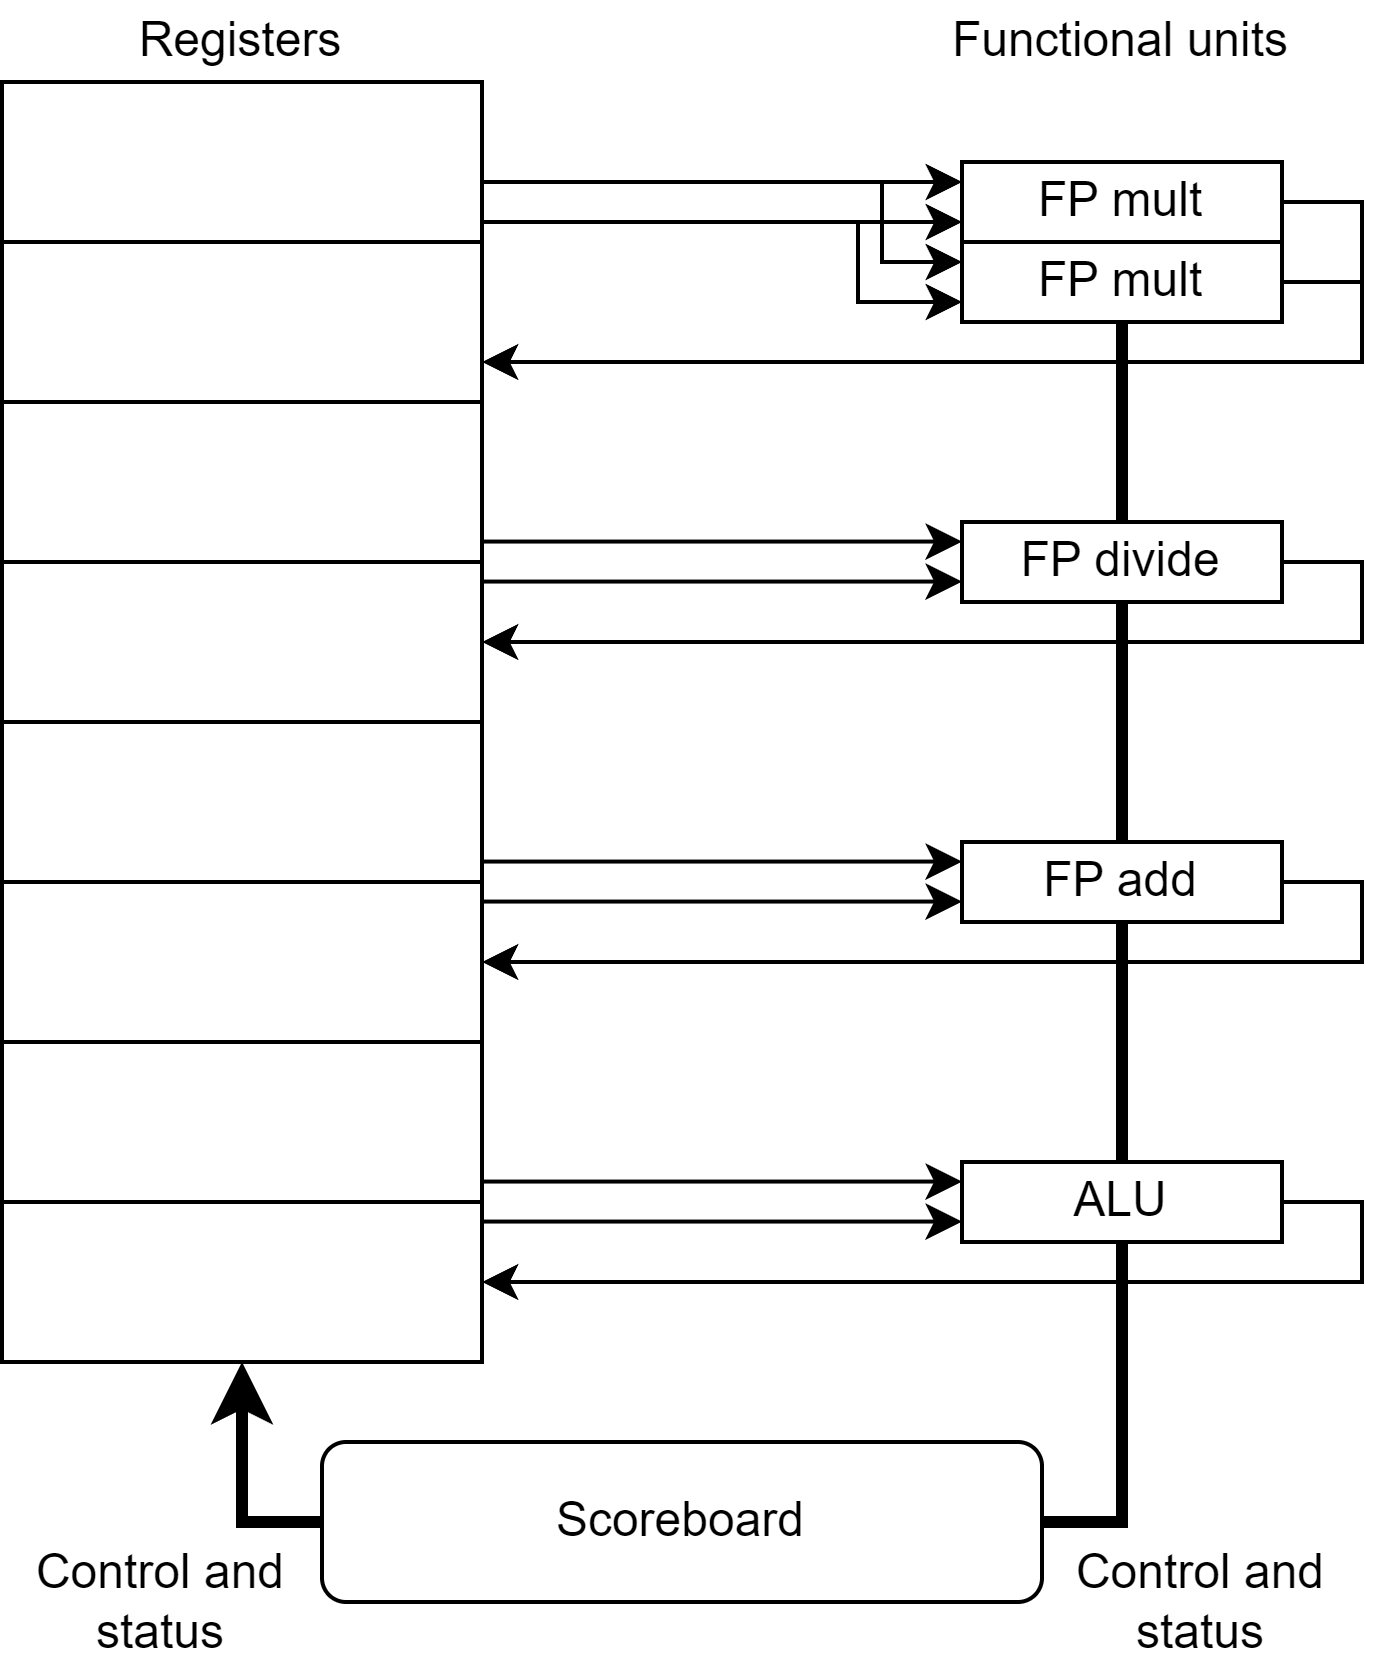
\includegraphics[width=0.5\linewidth]{images/cdc6600.png}
    \caption{CDC6600 Scoreboard}
\end{figure}
Scoreboard serves as the central hub for hazard management in the pipeline architecture. 
All instructions are routed through Scoreboard for processing.
It orchestrates the timing for instructions to access their operands and commence execution, continuously monitoring hardware changes to resolve stalled instructions. 
Additionally, it governs the timing for instructions to commit their results, optimizing performance and ensuring efficient instruction flow within the updated pipeline framework.

Scoreboard plays a crucial role in managing hazards and dependencies in the instruction pipeline. 
Without register renaming, it must detect WAW hazards and stall the issuance of new instructions until the conflicting instruction completes execution.
To accommodate multiple instructions in the execution phase, the system requires either multiple execution units or pipelined execution units. 
Scoreboard maintains the state of operations and tracks dependencies to ensure correct execution sequencing and hazard detection.

\subsection{Scoreboard structure}
The ID stage stage is now divided into two distinct phases:
\begin{enumerate}
    \item \textit{Issue}: this phase is responsible for instruction decoding and checking for structural hazards.
    \item \textit{Read operands}: this phase holds instructions until data hazards are resolved, with an out-of-order execution approach.
\end{enumerate}
Although instructions are issued sequentially, operand reading occurs out of order. 
This innovative approach, facilitated by Scoreboard, allows instructions without dependencies to execute, enhancing overall efficiency and throughput.

The structure of Scoreboard consists of several components:
\begin{enumerate}
    \item \textit{Instruction status}.
    \item \textit{Functional Unit status}: this indicates the state of each FU. 
    \item \textit{Register result status}: Indicates which FU will write to each register. 
        If no pending instructions will write to a register, this field is left blank.
\end{enumerate}

\subsection{Scoreboard control}
The four stages of Scoreboard control are:
\begin{enumerate}
    \item \textit{Issue}: during this stage, instructions are decoded and checked for structural hazards. 
        Instructions are dispatched to the functional unit if the corresponding unit is available and no other active instruction has the same destination register (avoiding WAW hazards). 
        If a structural hazard or a WAW hazard is detected, instruction issuance is stalled until these hazards are resolved.
    \item \textit{Reading operands}: in this stage, instructions wait until there are no data hazards before reading operands. 
        A source operand is considered available if no earlier issued active instruction will modify it, or if a functional unit is currently writing its value into a register.
        Once the source operands are available, Scoreboard instructs the functional unit to read the operands from the registers and begin execution. 
        RAW hazards are dynamically resolved during this stage, enabling out-of-order execution. This model does not involve data forwarding.
    \item \textit{Execution}: the functional unit begins operations on the provided operands. 
        Upon completing the operation, it informs Scoreboard about the execution's conclusion. 
        FUs are defined by their latency (the time required to complete one operation effectively) and their initiation interval (the number of cycles necessary between issuing two operations to the same FU).
    \item \textit{Write result}: after execution completion, Scoreboard checks for WAR hazards. 
        If no WAR hazards are detected, the results are written. 
        If a WAR hazard is identified, the instruction is stalled. 
        The design assumes overlap between issuing instructions and writing results is permitted.
\end{enumerate}

\subsection{Summary}
The core idea behind Scoreboard is to enable instructions behind a stall to proceed, allowing for the decoding, issuing, and reading of operands. 
This design achieves a speedup of 2.5 compared to systems without dynamic scheduling and a speedup of 1.7 by reorganizing instructions at the compiler level. 
However, the benefits are constrained by the slow memory (lacking cache) of CDC 6600.

Limitations of CDC 6600 Scoreboard include the lack of forwarding hardware, limitation to instructions within a basic block (leading to a small window), a limited number of FUs (particularly in integer and load and store units, leading to structural hazards), the inability to issue instructions on structural hazards, waiting for WAR hazards, and measures to prevent WAW hazards.